\chapter{运行试验和结果分析}\label{chap:run-analysis}

\section{部分运行结果对比}
\textbf{Lock Server}

\rltla 对规约 Lock Server 得到的归纳不变式如下:
\begin{lstlisting}
LockServerInd == 
    /\ TypeOK 
    /\ Inv
    /\ \A VARS \in Server : \A VARC \in Client : ~(VARS \in clientlocks[VARC]) \/ (~(semaphore[VARS])) 
\end{lstlisting}
所需时间: 20.43s

人工得到的归纳不变式如下:
\begin{lstlisting}
    Ind == 
        /\ TypeOK
        /\ Inv
        /\ \A c \in Client, s \in Server : (s \in clientlocks[c]) => ~semaphore[s]
\end{lstlisting}


\textbf{TwoPhase}
\begin{lstlisting}
TwoPhaseInd ==
    /\ TypeOK
    /\ TCConsistent
    /\ \A rmi \in RM : \A rmj \in RM : ~([type |-> "Abort"] \in msgs) \/ (~(rmState[rmi] = "committed"))
    /\ \A rmi \in RM : \A rmj \in RM : ([type |-> "Prepared", rm |-> rmi] \in msgs) \/ ((rmState[rmi] = "aborted") \/ (~(tmPrepared = RM)))
    /\ \A rmi \in RM : \A rmj \in RM : ([type |-> "Commit"] \in msgs) \/ (~(rmState[rmi] = "committed"))
    /\ \A rmi \in RM : \A rmj \in RM : ~(rmState[rmi] = "working") \/ (~(tmPrepared = tmPrepared \cup {rmi}))
    /\ \A rmi \in RM : \A rmj \in RM : ~([type |-> "Prepared", rm |-> rmi] \in msgs) \/ (~(rmState[rmi] = "working"))
    /\ \A rmi \in RM : \A rmj \in RM : (tmPrepared = tmPrepared \cup {rmi}) \/ (~(rmState[rmj] = "committed"))
    /\ \A rmi \in RM : \A rmj \in RM : ([type |-> "Prepared", rm |-> rmi] \in msgs) \/ (~(rmState[rmi] = "prepared"))
    /\ \A rmi \in RM : \A rmj \in RM : ([type |-> "Prepared", rm |-> rmj] \in msgs) \/ (~(tmPrepared = RM))
    /\ \A rmi \in RM : \A rmj \in RM : (tmPrepared = tmPrepared \cup {rmi}) \/ (~([type |-> "Commit"] \in msgs)) \/ (~(rmState[rmj] = "prepared"))
    /\ \A rmi \in RM : \A rmj \in RM : ([type |-> "Prepared", rm |-> rmi] \in msgs) \/ ((rmState[rmj] = "aborted") \/ (~([type |-> "Commit"] \in msgs)))
    /\ \A rmi \in RM : \A rmj \in RM : ([type |-> "Prepared", rm |-> rmi] \in msgs) \/ (~(tmPrepared = tmPrepared \cup {rmi}))
    /\ \A rmi \in RM : \A rmj \in RM : ~([type |-> "Abort"] \in msgs) \/ (~([type |-> "Commit"] \in msgs))
    /\ \A rmi \in RM : \A rmj \in RM : (tmState = "init") \/ (~(rmState[rmj] = "aborted")) \/ (~([type |-> "Commit"] \in msgs))
    /\ \A rmi \in RM : \A rmj \in RM : ([type |-> "Prepared", rm |-> rmi] \in msgs) \/ (~([type |-> "Commit"] \in msgs))
    /\ \A rmi \in RM : \A rmj \in RM : ~(rmState[rmj] = "committed") \/ (~(tmState = "init"))
    /\ \A rmi \in RM : \A rmj \in RM : (tmPrepared = tmPrepared \cup {rmi}) \/ (~([type |-> "Commit"] \in msgs))
    /\ \A rmi \in RM : \A rmj \in RM : (rmState[rmi] = "committed") \/ (~([type |-> "Commit"] \in msgs) \/ (~(rmState[rmi] = "aborted")))
    /\ \A rmi \in RM : \A rmj \in RM : ~([type |-> "Prepared", rm |-> rmi] \in msgs) \/ (~(rmState[rmi] = "aborted")) \/ (~(tmState = "init"))
    /\ \A rmi \in RM : \A rmj \in RM : ~([type |-> "Abort"] \in msgs) \/ (~(rmState[rmj] = "aborted")) \/ (~(tmState = "init"))
    /\ \A rmi \in RM : \A rmj \in RM : ~([type |-> "Abort"] \in msgs) \/ (~(tmState = "init"))
\end{lstlisting}
所需时间: 680.43s。

附录\ref{app:endive_TwoPhase}展示了endive 对此的归纳不变式结果。

\section{其他协议上的运行结果及与endive 对比分析}
除了以上两个典型规约,我们还在endive 提供的其他规约上运行了实验,结果如表\ref{tab:result}所示。
我们主要关注运行时间和\rltla 与endive对同一规约生成的归纳不变式的长度。
\begin{table}[!htbp]
	\centering
	\caption{其他协议上的实验结果}
	\renewcommand\arraystretch{1.4}
	\begin{tabular}{p{0.25\textwidth}p{0.25\textwidth}p{0.25\textwidth}p{0.15\textwidth}}
         \toprule
         \textbf{协议名称} &\textbf{RlTLA引理不变式数量} & \textbf{endive中引理不变式的数量}& \textbf{运行时间(s)}\\
         \midrule
         client server ae & 2 & 1 & 50.67\\
         quorum leader election& 2& 1 &30.74\\
         simple& 6& 1 &50.85\\
         toy consensus forall & 7 & 2&50.36  \\ 
         toy consensus epr & 5 & 3 &102.41  \\ 
         majorityset leader election& 2& 3 &36.74\\
         simple decentralized lock& 5 & 3 &372.32\\
         lock serv& 10 & 8 & 310.55\\
         \bottomrule
	\end{tabular}
	\label{tab:result}
\end{table}

对比endive的结果,相较而言,我们的工具生成归纳不变式寻找的引理不变式更多,效率较低。
对于这一现象的现象的解释,我认为是强化学习智能体在一开始尝试时会更偏向于选择已有的不变式比较相似的不变式,
但是在系统的提示下,相似的不变式往往不能得到很好的奖励值,于是系统便会在更加稀疏的区域寻找不变式。
并且没有考虑每个不变式所能消除的归纳反例的数量,只要某个不变式能消除归纳反例,就会被加入。
而endive则是通过基于候选不变式能杀死归纳反例的个数进行选择,事实上,它可能验证的不变式的个数更多。
这样的结果导致了,我们的工具会生成更多的相近不变式,但是,这不妨碍我们的工具生成最终正确的归纳不变式。

另外,系统运行的总体时间相较于endive偏长。
这是因为TLC和apalache没有直接的python接口,我们需要通过调用命令行的方式来调用TLC和apalache,并通过字符串解析命令行输出。
一次校验的时间,平均在0.3秒左右。相较于endive 一次校验数十个不变式,我们的工具一次校验一个不变式,所以时间上会有所增加。
但相较于随机遍历,以\textit{simple\_election}为例,拥有12个用户定义谓词,对于长度小于4的候选不变式,大概需要遍历接近万次。
然而我们的工具,遍历的次数在千次左右,在效率上有显著的提升。

\section{对比随机结果的消融实验}
为了证明强化学习模块在归纳不变式生成过程中起到了作用,我们在Two Phase协议上进行了强化学习模块的消融实验,我们使用完全随机的seed选择过程代替强化学习。
图\ref{fig:all}展示我们的实验结果,其中,图\ref{fig:inv}表示截至目前为止,每轮生成的候选引理不变式通过不变式检查的频率,图\ref{fig:ind}表示最终加入到归纳不变式候选集合中的概率。
以上图表表明,强化学习模块在归纳不变式生成过程中起到了积极的作用,提高了候选引理不变式的质量。
\begin{figure}[htb]
    \centering
    \subfloat[invaraint hit rate]{
        \label{fig:inv}
        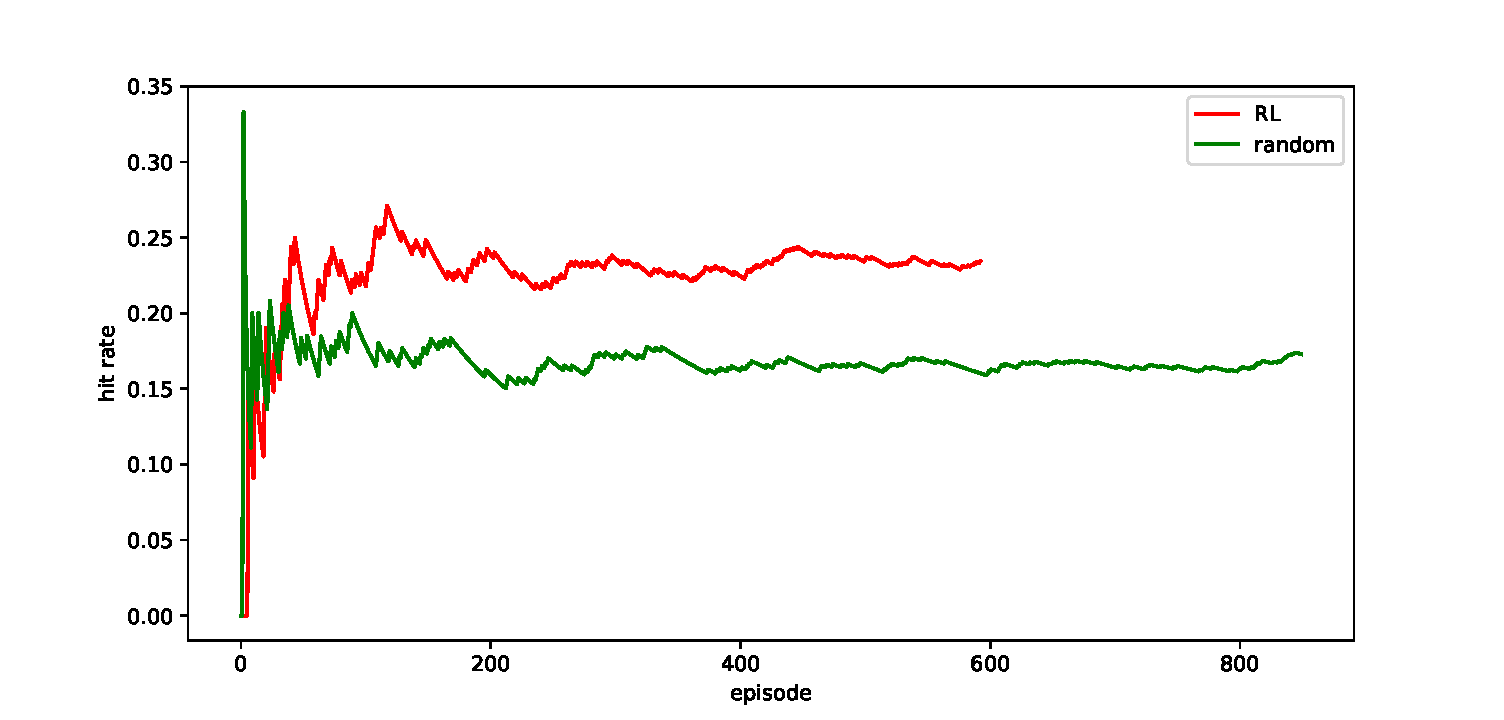
\includegraphics[width=0.8\linewidth]{figures/inv.pdf}
    }\hfill
    \subfloat[inductive invariant hit rate]{
        \label{fig:ind}
        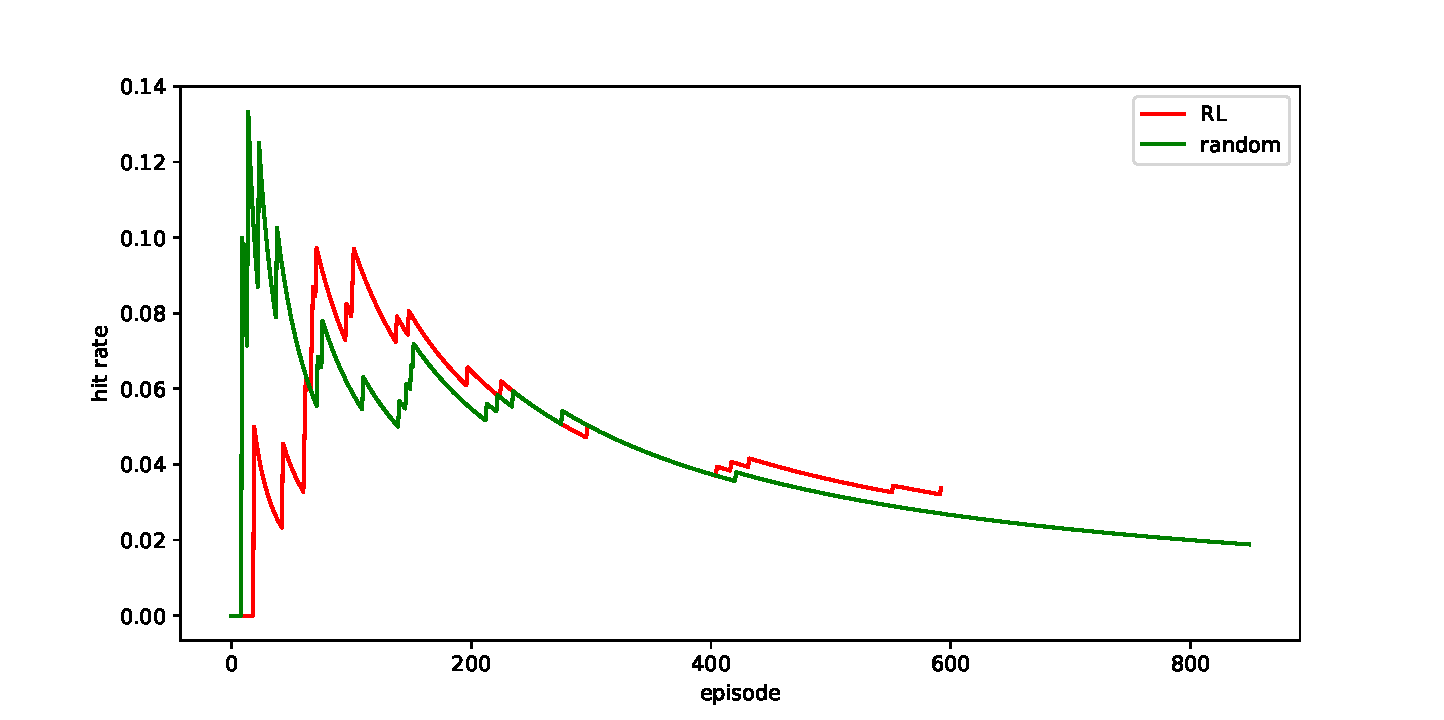
\includegraphics[width=0.8\linewidth]{figures/ind.pdf}
    }\hfill
    \caption{强化学习选择和随机选择的命中率}
    \label{fig:all}
\end{figure}
